\chapter{Introduzione alla programmazione lineare a numeri interi}

Si consideri il seguente problema.
\begin{flalign}
	& Min\;cx \\
	& \;\;\;\;\;\;\;Ax=b \\
	& \;\;\;\;\;\;\;x\ge 0 \\
	& \;\;\;\;\;\;\;x\;intero
\end{flalign}
Le variabili devono assumere valori interi:
\begin{flalign}
	& Es:\;\;x_{i}=Numero\;di\;uomini\;che\;devono\;essere\;assegnati\;al\;lavoro\;i. \\
	& \;\;\;\;\;\;\;\;\;\;\;\;\;=Numero\;di\;automezzi\;che\;devono\;operare\;il\;trasporto\;lungo\;la\;"tratta\; i". \\
\end{flalign}

\section{Arrotondamento ad una soluzione non-intera}
Si risolva il problema ignorando i vincoli [$x: intero$].
Le variabili che risultano non intere, nella soluzione ottima del problema continuo, vengano arrotondate al valore intero pi\`u vicino.
\begin{flalign}
	& Es:\;\;Min\;z=-2x_{1}+3x_{2} \\
	& \;\;\;\;\;\;\;\;\;\;x_{1}+x_{2}\ge 3 \\
	& \;\;\;\;\;\;\;\;\;\;3x_{1}+x_{2}\le 6 \\
	& \;\;\;\;\;\;\;\;\;\;x_{2}\le 5 \\
	& \;\;\;\;\;\;\;\;\;\;x_{1},\;x_{2}\ge 0\;ed\;intere
\end{flalign}
\begin{figure}[h]
	\centering
	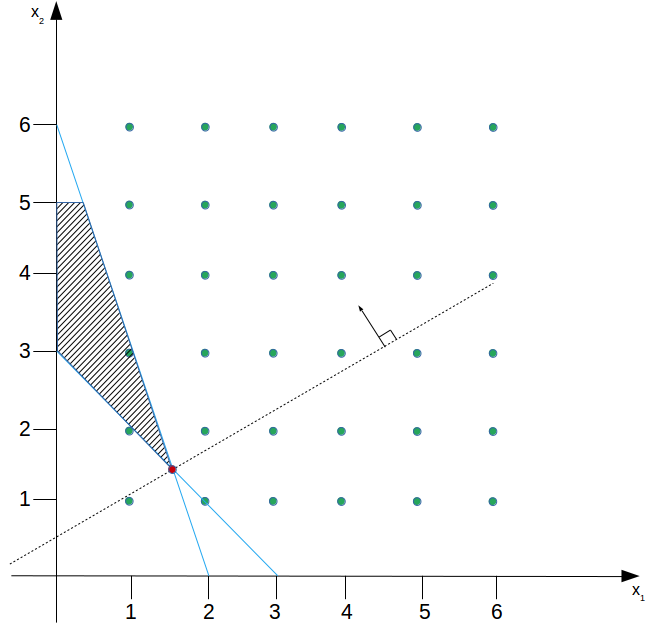
\includegraphics[height=12cm]{images/graph6.png}
	\label{fig:SoluzioneOttimaContinua1}
	\caption[]{\\Soluzione continua: $z=\frac{3}{4}$; $x_{1}=\frac{3}{2}$, $x_{2}=\frac{3}{2}$ \\ Soluzione intera: $z=4$; $x_{1}=1$, $x_{2}=2$}
\end{figure}

In questo esempio la soluzione arrotondata coincide con la soluzione ottima.

\begin{flalign}
& Es:\;\;Min\;z=8x_{1}+6x_{2} \\
& \;\;\;\;\;\;\;\;\;\;4x_{1}+3x_{2}\ge 6 \\
& \;\;\;\;\;\;\;\;\;\;x_{1},\;x_{2}\ge 0\;ed\;intere
\end{flalign}
\begin{figure}[h]
	\centering
	\captionsetup{justification=centering}
	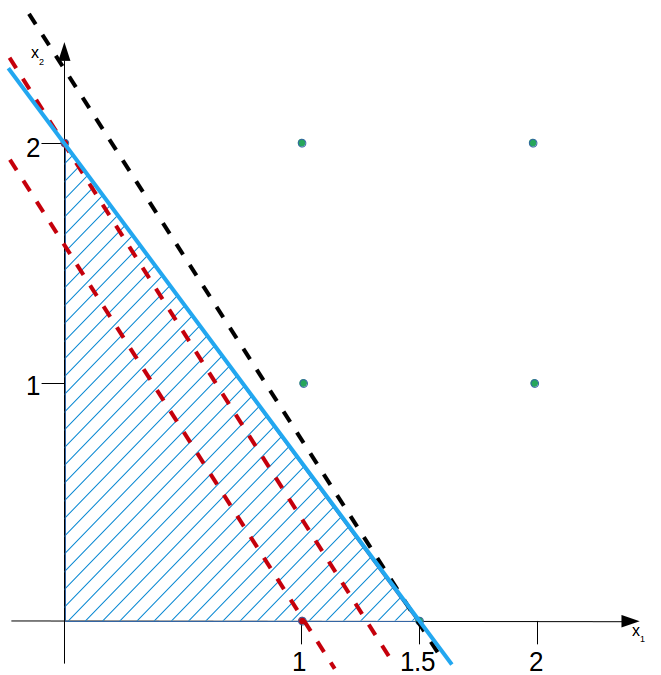
\includegraphics[height=13cm]{images/graph7.png}
	\label{fig:SoluzioneOttimaContinua2}
	\caption[]{\\ Soluzione continua: $z=12$; $x_{1}=1,5$, $x_{2}=0$ \\ Soluzione arrotondata $z=8$; $x_{1}=1$, $x_{2}=0$ \\ Soluzione intera: $z=10$; $x_{1}=0$, $x_{2}=2$}
\end{figure}

La soluzione arrotondata si discosta notevolmente dalla soluzione ottima.

\begin{flalign}
& Es:\;\;Min\;z=8x_{1}+6x_{2} \\
& \;\;\;\;\;\;\;\;\;\;4x_{1}+3x_{2}\ge 6 \\
& \;\;\;\;\;\;\;\;\;\;x_{1},\;x_{2}\ge 0\;ed\;intere
\end{flalign}
\begin{figure}[h]
	\centering
	\captionsetup{justification=centering}
	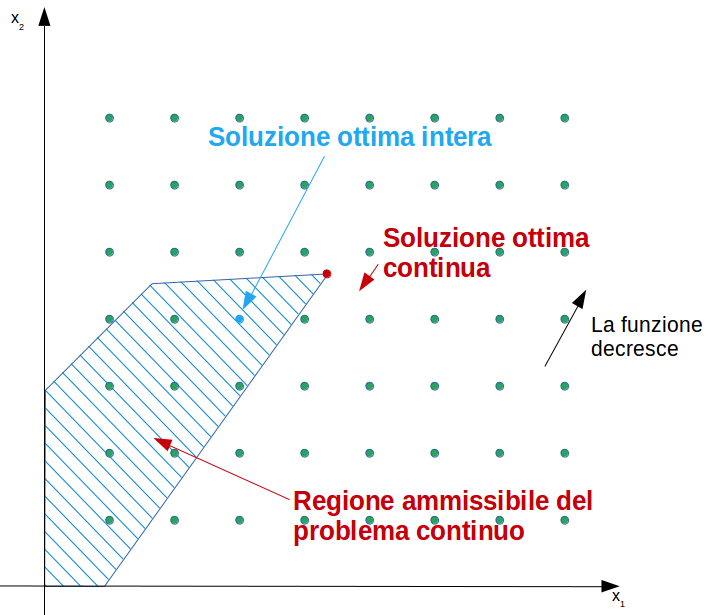
\includegraphics[height=14cm]{images/graph8.png}
	\label{fig:SoluzioneOttimaContinua3}
\end{figure}

I quattro punti interi pi\`u vicini alla soluzione continua non sono ammissibili.
\newpage

\section{Unimodularit\`a}
La matrice intera A di $m$ righe ed $n$ colonne \`e totalmente unimodulare se ogni sua sottomatrice quadrata B non singolare \`e unimodulare, ovvero $det(B)=\pm 1$.
\newline

\textbf{Teorema.} Se la matrice intera $A$ \`e totalmente unimodulare allora tutti i punti estremi dell'insieme pd. convesso $X={x:\;Ax=b,\;x\ge 0}$ sono interi per ogni vettore intero $b$.
\newline

\textbf{Dimostrazione.} Sia B una base ammissibile e $x_{b}$ le variabili base: $Bx_{B}=b$.\newline Per la regola di Cramer:
\begin{flalign}
	& x_{b_{i}}=\frac{\det(B_{i})}{\det(B)}
\end{flalign}
Dove $B_{i}$ si ottiene da $B$ sostituendo la i-esima colonna di $B$ con $b$. \`E ovvio che $\det(B_{i})$ \`e un numero intero e quindi anche ciascun $x_{B_{i}}$ \`e intero.
\newline

\textbf{Teorema.} Una matrice intera $A$ i cui elemento sono $0, +1, -1$ \`e totalmente unimodulare se:
\begin{enumerate}
	\item In ogni colonna $A$ compaiono al pi\`u due elementi non-nulli (cioè $1,-1$);
	\item L'insieme delle righe R pu\`o essere suddiviso in due insieme disgiunti $R_{1}$ e $R_{2}$ ($R_{1}\cup R_{2}=R$) per cui:
	\begin{enumerate}
		\item Se una colonna contiene due elementi non-nulli dello stesso segno allora la riga corrispondente ad uno dei due elementi appartiene a $R_{1}$ mentre la riga relativa all'altro elemento \`e in $R_{2}$;
		\item Se una colonna contiene due elementi di segno opposto entrambe le righe appartengono allo stesso insieme.
	\end{enumerate}
\end{enumerate}

\textbf{Esempi.}
\newline

\begin{tabular}{cc}
	$ A=\begin{bmatrix}
		-1 & 1 & 1 & 0 & 0 & 0 \\
		0 & 0 & -1 & -1 & 1 & 1 \\
		0 & 0 & 0 & 0 & 0 & -1 \\
		1 & -1 & 0 & 1 & -1 & 0 \\
	\end{bmatrix},$ &
	$A = \begin{bmatrix}
		-1 & 1 & 1 & 0 & 0 & 0 \\
		0 & 0 & -1 & -1 & 1 & 1 \\
		0 & 0 & 0 & 0 & 0 & -1 \\
		1 & -1 & 0 & 1 & -1 & 0 \\
	\end{bmatrix}$ \\
	\begin{minipage}{0pt}
		\vskip 10pt
		\begin{itemize}
			\item[$R={1,2,3,4}$]
			\item[$R_{1}={1,2,3,4}$]
			\vspace{-6mm}
			\item[$R_{2}=\emptyset$]
			\vspace{-6mm}
		\end{itemize}
	\end{minipage} &
	\begin{minipage}{0pt}
		\vskip 10pt
		\begin{itemize}
			\item[$R={1,2,3,4,5}$]
			\item[$R_{1}={1,2,3}$]
			\vspace{-6mm}
			\item[$R_{2}={4,5}$]
			\vspace{-6mm}
		\end{itemize}
	\end{minipage} \\
\end{tabular}

La totale unimodularit\`a della matrice $A$ \`e \textbf{condizione sufficiente} affinch\`e la soluzione ottima $x^{*}$ sia intera per
\begin{flalign*}
	& Min\;cx\\
	& \;\;\;\;\;\;\;\;Ax=b\;(b intero)\\
	& \;\;\;\;\;\;\;\;x\ge 0
\end{flalign*}
La condizione non \`e \textbf{necessaria}.\newline\newline
\textbf{Esempio:}

dato il sistema di vincoli
\begin{flalign*}
	& 6x_{1}+x_{2}=7 \\
	& 2x_{1}+x_{2}=3
\end{flalign*}
L'unica soluzione \`e ($x_{1}=1,\;x_{2}=1$) mentre la matrice
\begin{center}
	$ A=\begin{bmatrix}
	6 & 1 \\
	2 & 1
	\end{bmatrix}$	
\end{center}
non risulta essere totalmente unimodulare.
\newpage

\section{Metodo dei piani di taglio}
Sia dato il problema
\begin{displaymath}
ILP
	\begin{cases}
	\;Min\;z_{ILP}=cx\\
	\;\;\;\;\;\;\;\;\;\;\;\;\;\;\;\;\;\;\;\;\;A x = b\\
	\;\;\;\;\;\;\;\;\;\;\;\;\;\;\;\;\;\;\;\;\;x \ge 0\;e\:intero
	\end{cases}
\end{displaymath}

Supponiamo A,c,b interi.

Si consideri il problema rilassato che si ottiene da 'ILP' ignorando i vincoli di interezza. Indichiamo tale problema con \textbf{\emph{LP}}.
\begin{displaymath}
	LP
	\begin{cases}
	\;z_{LP}\;=\;Min\;cx\\
	\;\;\;\;\;\;\;\;\;\;\;\;\;\;\;\;\;\;\;\;\;\;ax=b\\
	\;\;\;\;\;\;\;\;\;\;\;\;\;\;\;\;\;\;\;\;\;\;x\ge 0\\
	\end{cases}
\end{displaymath}

\`E noto che $z_{LP}\le z_{ILP}$.

\subsection{Piani di taglio}
Si risolva $LP$; se la soluzione è intera tale soluzione è anche l'ottimo di $ILP$.

Altrimenti vengono aggiunti a $LP$ vincoli, \emph{che non escludono soluzioni intere}, fino a che la soluzione del problema $LP$ risultante non risulti intera.

\begin{figure}[!htb]
	\minipage{0.32\textwidth}
	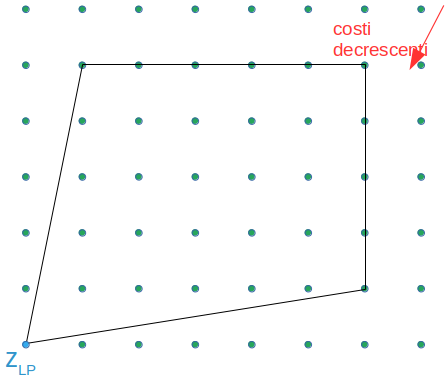
\includegraphics[width=\linewidth]{images/graph9.png} 
	(A)
	\label{fig:pianiditaglio1}
	\endminipage\hfill
	\minipage{0.32\textwidth}
	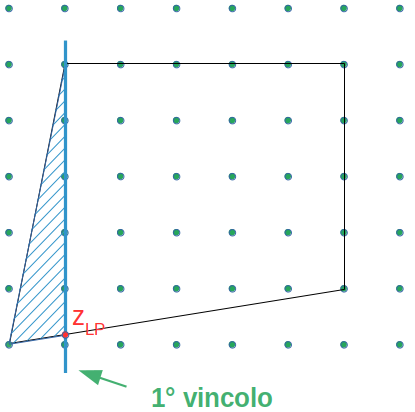
\includegraphics[width=\linewidth]{images/graph10.png}
	(B)
	\label{fig:pianiditaglio2}
	\endminipage\hfill
	\minipage{0.32\textwidth}%
	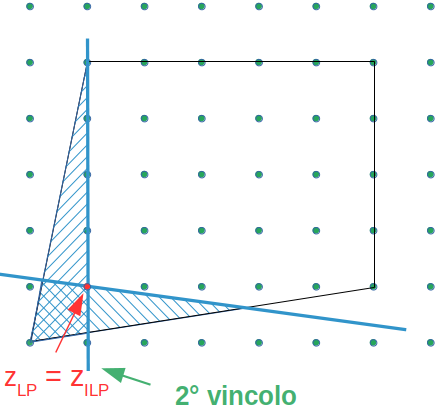
\includegraphics[width=\linewidth]{images/graph11.png}
	(C)
	\label{fig:paniditaglio3}
	\endminipage
\end{figure}

In $(A)$ viene mostrata la regione ammissibile di $LP$ ed il punto di ottimo.

In $(B)$ viene mostrata la regione ammissibile di $LP$ più un vincolo che rende non-ammissibile l'ottimo ottenuto in $(A)$ ma che non esclude nessuno dei punti interi.

In $(C)$ viene mostrato come l'aggiunta di un secondo vincolo rende la soluzione intera.
\newline
\newline
\textbf{Nell'esempio sono sufficienti 2 vincoli per rendere la soluzione intera.}
\newline
\newline
In generale bisogna aggiungere vincoli fino a che la soluzione non risulti intera o si scopra che il problema non ha soluzioni intere.

\subsection{Gomory cuts}
Si consideri il tableau ottimo relativo a LP:

\begin{table}[h]
	\centering
	\begin{tabular}{llllllllllllll}
		&                       z & $x_{1}$ &    & ... &     &      & $x_{m}$ & $x_{m+1}$     & ... & $x_{j}$     & ... & $x_{n}$     & \\ \cline{2-14}
		& \multicolumn{1}{|l|}{1} & 0       &    & ... &     &      & 0       &               &     &             &     &             & \multicolumn{1}{|l|}{} \\ \cline{2-14}
		$x_{1}$ & \multicolumn{1}{|l|}{}  & 1       &    &     &     &      &         &               &     &             &     &	           & \multicolumn{1}{|l|}{$\bar{b}_{1}$} \\
		& \multicolumn{1}{|l|}{}  &         & 1  &     &     &      &         &               &     &             &     &             & \multicolumn{1}{|l|}{} \\
		& \multicolumn{1}{|l|}{}  &         &    & ... &     &      &         &               &     &             &     &             & \multicolumn{1}{|l|}{} \\
		$x_{r}$ & \multicolumn{1}{|l|}{}  &         &    &     & 1   &      &         & $y_{r}^{m+1}$ & ... & $y_{r}^{j}$ & ... & $y_{r}^{n}$ & \multicolumn{1}{|l|}{$\bar{b}_{r}$} \\
		& \multicolumn{1}{|l|}{}  &         &    &     &     & ...  &         &               &     &             &     &             & \multicolumn{1}{|l|}{} \\
		$x_{m}$ & \multicolumn{1}{|l|}{}  &         &    &     &     &      & 1       &               &     &             &     &             & \multicolumn{1}{|l|}{$\bar{b}_{m}$} \\ \cline{2-14}
	\end{tabular}
\end{table}

Supponiamo la soluzione ottima non intera.\newline

\emph{Sia $\bar{b}_{r}$ non intero.}
\newline

L'equazione associata a $x_{r}$ è:

\begin{equation}\label{eq:2.20}
x_{r} + \sum_{j=m+1}^{n} y_{r}^{j} x_{j} = \bar{b}_{r}
\end{equation}

Poniamo:
\begin{equation}
y_{r}^{j} = I_{r}^{j} + F_{r}^{j}\text{, dove }I_{r}^{j} = \lfloor y_{r}^{j} \rfloor,\;(0 \le F_{r}^{j} < 1)
\end{equation}

Inoltre:
\begin{equation}
\bar{b}_{r} = I_{r} + F_{r} \text{ essendo } 0 \le F_{r} < 1
\end{equation}

Sostituendo, la \ref{eq:2.20} diviene:
\begin{equation}
x_{r} + \sum_{j=m+1}^{n} (I_{r}^{j} + F_{r}^{j}) x_{j} = (I_{r} + F_{r})
\end{equation}

o anche:
\begin{equation}
\underbrace{x_{r}+\sum_{j=m+1}^{n} I_{r}^{j} x_{j} - I_{r}}_\text{intero per ogni x intero} = \underbrace{F_{r} - \sum_{j=m+1}^{n} F_{r}^{j}x_{j}}_\text{< 1 per $x\ge0$}
\end{equation}

Ne segue:

\begin{equation}
F_{r} - \sum_{j=m+1}^{n} F_{r}^{j} x_{j} \le 0
\end{equation}

\noindent
La soluzione corrente non soddisfa il vincolo \ref{eq:2.20} in quanto $x_{j} = 0$ $j=m+1,...,n$ mentre $F_{r}>0$ poiché $\bar{b}_{r}$ si è supposto non intero.

Se il vincolo \ref{eq:2.20} viene aggiunto al problema $LP$ allora la soluzione corrente risulterà non ammissibile.\newline
Per determinare una nuova soluzione che soddisfi il vincolo \ref{eq:2.20} può essere impiegato il \emph{Simplesso Duale} partendo dal tableau ottimo relativo alla soluzione corrente.
\newline

\noindent
Al tableau va aggiunto il vincolo:
\begin{equation}
- \sum_{j=m+1}^{j} F_{r}^{j} x_{j} + s = -F_{r}
\end{equation}
La nuova variabile slack $s$ è una nuova variabile base.\newline
Il nuovo tableau è non ammissibile per il Primale ma duale ammissibile.\newline

\noindent
\textbf{Esempio.}

\begin{flalign*}
& Min\; - x_{2} \\
& \;\;\;\;\;\;\;\;\;3x_{1}+2x_{2}\le 6 \\
& \;\;\;\;\;-3x_{1}+2x_{2}\le 0 \\
& \;\;\;\;\;\;\;\;\;x_{1},\;x_{2}\ge 0 \\
& \;\;\;\;\;\;\;\;\;x_{1},\;x_{2}\;intere\;\ge 0 \\
\end{flalign*}
Si noti che l'ottimo cade nel punto $x=(1;1)$.

\centerline{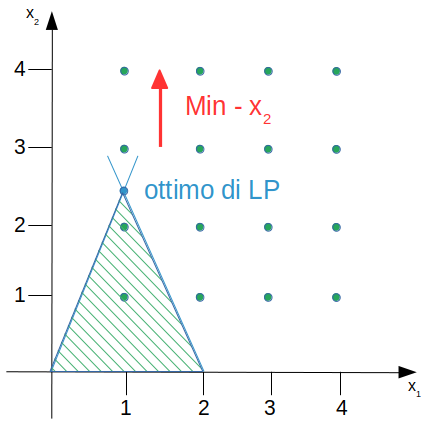
\includegraphics[height=9cm]{images/graph12.png}}

\begin{table}[h]
	\centering
	\begin{tabular}{lllllll}
				&                       z & $x_{1}$ & $x_{2}$  & $x_{3}$ & $x_{4}$ &  RHS  \\ \cline{2-7}
			z	& \multicolumn{1}{|l|}{1} & 0       & 1        & 0       & 0       & \multicolumn{1}{|l|}{0} \\ \cline{2-7}
		$x_{3}$ & \multicolumn{1}{|l|}{0} & 3       & 2        & 1       & 0	   & \multicolumn{1}{|l|}{6} \\
		$x_{4}$ & \multicolumn{1}{|l|}{0} & -3      & \textcircled{2}        & 0       & 1       & \multicolumn{1}{|l|}{0} \\ \cline{2-7}
	\end{tabular}
\end{table}

\begin{table}[!h]
	\centering
	\begin{tabular}{lllllll}
		        &                       z & $x_{1}$ & $x_{2}$  & $x_{3}$ & $x_{4}$ &  RHS  \\ \cline{2-7}
		      z & \multicolumn{1}{|l|}{1} & 3/2     & 0        & 0       & -1/2    & \multicolumn{1}{|l|}{0} \\ \cline{2-7}
		$x_{3}$ & \multicolumn{1}{|l|}{0} & \textcircled{6}   & 0       & 1 & -1  & \multicolumn{1}{|l|}{6} \\
		$x_{2}$ & \multicolumn{1}{|l|}{0} & -3/2    & 1        & 0       & 1/2     & \multicolumn{1}{|l|}{0} \\ \cline{2-7}
	\end{tabular}
\end{table}

\begin{table}[!h]
	\centering
	\begin{tabular}{lllllll}
				&                         & $x_{1}$ & $x_{2}$  & $x_{3}$ & $x_{4}$ &  RHS  \\ \cline{2-7}
			z	& \multicolumn{1}{|l|}{1} & 0       & 0        & -1/4    & -1/4    & \multicolumn{1}{|l|}{-3/2} \\ \cline{2-7}
		$x_{1}$ & \multicolumn{1}{|l|}{0} & 1       & 0        & 1/6     & -1/6    & \multicolumn{1}{|l|}{1} \\
		$x_{2}$ & \multicolumn{1}{|l|}{0} & 0       & 1        & 1/4     & 1/4     & \multicolumn{1}{|l|}{3/2} \\ \cline{2-7}
	\end{tabular}
	\caption{Tableau ottimo. Soluzione continua!}
\end{table}

Ricordando che il cut da aggiungere è:
\begin{equation}
-\sum_{j=m+1}^{n} F_{r}^{j} x_{j} + s = -F_{r}
\end{equation}
Dalla riga di $x_{2}$ si ha la sequente equzione:
\begin{equation}
	x_{2} + \frac{1}{4} x_{3} + \frac{1}{4} x_{4} = \frac{3}{2}
\end{equation}
da cui:
\begin{equation}\label{eq:2.29}
-\frac{1}{4}x_{3} - \frac{1}{4} x_{4} + s_{1} = -\frac{1}{2} 
\end{equation}

Si osservi che per definizione di $x_{3}$ e $x_{4}$ si ha
\begin{equation}
x_{3} = 6 - 3x_{1} - 2x_{2}\text{ ed }x_{4} = 3x_{1} - 2x_{2}
\end{equation}
Sostituendo in \ref{eq:2.29} si ottiene $x_{2}\le 1$